%% The first command in your LaTeX source must be the \documentclass command.
%% Options: hf: enable header and footer.
\documentclass[
% twocolumn,
% hf,
]{ceurart}

%% One can fix some overfulls
%\sloppy


%% Minted listings support
%% Need pygment <http://pygments.org/> <http://pypi.python.org/pypi/Pygments>
\usepackage{minted}
%% auto break lines
\setminted{breaklines=true}

%%
%% end of the preamble, start of the body of the document source.
\begin{document}

%%
%% Rights management information.
%% CC-BY is default license.
\copyrightyear{2025} % Actualizado para REST-MEX 2025
\copyrightclause{Copyright for this paper by its authors.
  Use permitted under Creative Commons License Attribution 4.0
  International (CC BY 4.0).}

%%
%% This command is for the conference information
% \conference{IberLEF 2025: International Iberian Languages Evaluation Forum, September 2025, Spain.}
\conference{Proyecto Final - Cómputo Estadístico, CIMAT, 2025}


%%
%% The "title" command
\title{Inferencia Bayesiana de Puntos de Cambio y Riesgo en Bitcoin: JIT-MCMC vs. GJR-GARCH}
% \subtitle{Clasificación de Polaridad, Tipo de Destino e Identificación de Pueblos Mágicos} % Subtítulo opcional

% \tnotemark[1] % Si necesitas una nota para el título
% \tnotetext[1]{Este trabajo fue parcialmente financiado por XYZ.}

%%
%% The "author" command and its associated commands are used to define
%% the authors and their affiliations.

% --- Equipo ---
\author[1]{Gustavo Hernández-Angeles}[
orcid=0009-0001-3160-5294,
email=gustavo.hernandez@cimat.mx,
]\cormark[1] % Marca de autor de correspondencia

\author[1]{Javiere Tiscareño-Calzadilla}[
orcid=0009-0005-8418-7355,
email=cesar.aguirre@cimat.mx,
]

\author[1]{Diego Paniagua-Molina}[
orcid=0009-0006-6564-2794,
email=diego.paniagua@cimat.mx,
]


% --- Afiliaciones ---
\address[1]{Mathematics Research Center (CIMAT—Centro de Investigación en Matemáticas), Graduate Program in Statistical Computing, Nuevo León, Mexico}



%% Footnotes
\cortext[1]{Corresponding author.}
% \fntext[1]{Estos autores contribuyeron de igual manera (These authors contributed equally).}


%% The abstract is a short summary of the work to be presented in the
%% article.
\begin{abstract}
  Este proyecto investiga la dinámica de la volatilidad extrema en el mercado de Bitcoin (BTC-USD) durante el periodo 2019-2024. Se contrasta un enfoque econométrico robusto (GJR-GARCH con errores t-Student) frente a una metodología computacional intensiva basada en Inferencia Bayesiana (Change-Point Detection vía Gibbs Sampling). El diferenciador técnico reside en la optimización computacional mediante compilación Just-In-Time (JIT) con Numba y el uso de técnicas de Bootstrap para construir intervalos de confianza sobre las métricas de riesgo (VaR). Los resultados muestran que, aunque el modelo Bayesiano optimizado es computacionalmente eficiente, el modelo GJR-GARCH ofrece una mejor calibración del riesgo de cola según la prueba de Kupiec.
\end{abstract}

%%
%% Keywords. The author(s) should pick words that accurately describe
%% the work being presented. Separate the keywords with \sep.
\begin{keywords}
  Bitcoin \sep Volatilidad \sep GJR-GARCH \sep Gibbs Sampling \sep MCMC \sep Numba \sep Value at Risk \sep Change-Point Detection
\end{keywords}

%%
%% This command processes the author and affiliation and title
%% information and builds the first part of the formatted document.
\maketitle

%--------------------------------------------------------------------------
%	CUERPO DEL ARTÍCULO
%--------------------------------------------------------------------------

\section{Introduction}

Las series de tiempo de criptoactivos, como el Bitcoin (BTC) \cite{nakamoto2008bitcoin}, presentan desafíos únicos para el modelado financiero y la gestión de riesgos. A diferencia de los activos tradicionales, las criptomonedas exhiben una volatilidad extrema, ``colas pesadas'' (fat tails) y cambios de régimen abruptos impulsados por factores exógenos, regulatorios y tecnológicos. La correcta estimación del riesgo de mercado, cuantificado comúnmente a través del Valor en Riesgo (VaR), es crucial tanto para inversores institucionales como para el cumplimiento de normativas internacionales como Basilea III.

Los modelos econométricos clásicos, como el GARCH (Generalized Autoregressive Conditional Heteroskedasticity), asumen a menudo distribuciones normales que subestiman la probabilidad de eventos extremos. Variantes como el GJR-GARCH han sido propuestas para capturar asimetrías (efecto apalancamiento), pero su estimación suele basarse en máxima verosimilitud, lo cual puede ser inestable en muestras finitas o con ruido excesivo.

Como alternativa, la inferencia bayesiana ofrece un marco flexible para incorporar incertidumbre en los parámetros y modelar cambios estructurales explícitos. Sin embargo, los métodos de Monte Carlo vía Cadenas de Markov (MCMC) requeridos para su estimación son computacionalmente costosos, lo que ha limitado su adopción en aplicaciones de alta frecuencia.

El objetivo de este trabajo es implementar y comparar dos paradigmas de modelado:
\begin{enumerate}
    \item Un modelo econométrico robusto: \textbf{GJR-GARCH(1,1)} con errores t-Student.
    \item Un modelo bayesiano de \textbf{Detección de Puntos de Cambio} (Change-Point Detection) implementado mediante Gibbs Sampling.
\end{enumerate}

Para abordar el reto computacional del enfoque bayesiano, se propone una implementación optimizada utilizando compilación Just-In-Time (JIT) con la librería \texttt{Numba} en Python. Además, se emplean técnicas de Bootstrap de Bloques para generar intervalos de confianza para el VaR, permitiendo una validación estadística rigurosa más allá de la estimación puntual.

\section{Marco Teórico}

\subsection{Modelo GJR-GARCH con Errores t-Student}
El modelo GJR-GARCH, propuesto por Glosten, Jagannathan y Runkle \cite{glosten1993relation}, extiende el GARCH estándar para capturar la asimetría en la volatilidad: los retornos negativos (malas noticias) tienden a incrementar la volatilidad más que los retornos positivos (buenas noticias) de igual magnitud.

Sea $r_t = \mu + \epsilon_t$, donde $\epsilon_t = \sigma_t z_t$. La varianza condicional $\sigma_t^2$ evoluciona según:
\begin{equation}
\sigma_{t}^{2}=\omega+(\alpha+\gamma I_{t-1})\epsilon_{t-1}^{2}+\beta\sigma_{t-1}^{2}
\end{equation}
donde:
\begin{itemize}
    \item $\omega > 0, \alpha \ge 0, \beta \ge 0, \alpha + \gamma \ge 0$.
    \item $I_{t-1} = 1$ si $\epsilon_{t-1} < 0$, y $0$ en caso contrario.
    \item $\gamma$ captura el efecto de apalancamiento. Si $\gamma > 0$, los shocks negativos aumentan más la volatilidad.
\end{itemize}

Para modelar las colas pesadas características de Bitcoin, asumimos que las innovaciones estandarizadas $z_t$ siguen una distribución t-Student con $\nu$ grados de libertad, cuya función de densidad es:
\begin{equation}
f(z|\nu) = \frac{\Gamma(\frac{\nu+1}{2})}{\sqrt{\nu\pi}\Gamma(\frac{\nu}{2})} \left(1 + \frac{z^2}{\nu}\right)^{-\frac{\nu+1}{2}}
\end{equation}

\subsection{Modelo Bayesiano de Punto de Cambio (Change-Point)}
Se propone un modelo jerárquico donde la varianza de los retornos sufre un cambio estructural en un momento desconocido $k \in \{1, \dots, T\}$.
\begin{equation}
y_{t} \sim \mathcal{N}(0, \sigma_{t}^{2}), \quad \sigma_{t}^{2} = \begin{cases} \sigma_1^2 & \text{si } t \le k \\ \sigma_2^2 & \text{si } t > k \end{cases}
\end{equation}

\subsubsection{Especificación de Priors}
Se utilizan priores conjugados para facilitar el muestreo de Gibbs:
\begin{itemize}
    \item \textbf{Punto de cambio:} Prior uniforme discreta sobre el dominio temporal.
    \begin{equation}
    k \sim \mathcal{U}\{1, T\}
    \end{equation}
    \item \textbf{Varianzas:} Prior Inversa-Gamma para asegurar positividad.
    \begin{equation}
    \sigma_i^2 \sim \mathcal{IG}(\alpha, \beta), \quad i \in \{1, 2\}
    \end{equation}
\end{itemize}

\subsubsection{Inferencia vía Gibbs Sampling}
El algoritmo alterna entre muestrear las varianzas condicionales al punto de cambio y muestrear el punto de cambio condicional a las varianzas:
1. \textbf{Muestrear $\sigma_i^2 | k, \mathbf{y}$:} Dado $k$, los datos se dividen en dos grupos. La posterior es también Inversa-Gamma debido a la conjugación.
2. \textbf{Muestrear $k | \sigma_1^2, \sigma_2^2, \mathbf{y}$:} Se calcula la verosimilitud marginal para cada posible punto de corte $t$ y se muestrea de la distribución multinomial resultante.
\begin{equation}
P(k=t | \cdot) \propto \prod_{i=1}^t \mathcal{N}(y_i | 0, \sigma_1^2) \prod_{j=t+1}^T \mathcal{N}(y_j | 0, \sigma_2^2)
\end{equation}

\section{Análisis de Datos}

Se utilizaron datos históricos diarios de precios de cierre ajustados del par Bitcoin vs Dólar Estadounidense (BTC-USD), obtenidos a través de la API de Yahoo Finance. El periodo de análisis abarca desde el 1 de enero de 2019 hasta el 1 de enero de 2024, cubriendo eventos significativos como la crisis del COVID-19 (marzo 2020) y el colapso de FTX (noviembre 2022).

La serie de precios $P_t$ fue transformada a retornos logarítmicos diarios mediante la fórmula $r_{t}=100 \cdot (\ln(P_{t})-\ln(P_{t-1}))$. La Tabla \ref{tab:stats} presenta las estadísticas descriptivas de la serie.

\begin{table}[h]
\centering
\caption{Estadísticas Descriptivas de los Retornos Diarios de Bitcoin (\%)}
\label{tab:stats}
\begin{tabular}{lr}
\toprule
Estadístico & Valor \\
\midrule
Media & 0.13 \\
Desviación Estándar & 3.53 \\
Mínimo & -46.47 \\
Máximo & 17.18 \\
Asimetría (Skewness) & -1.22 \\
Curtosis (Kurtosis) & 18.96 \\
\bottomrule
\end{tabular}
\end{table}

Se observa una curtosis extremadamente alta (18.96), muy superior a la de una distribución normal (3.0), lo que confirma la presencia de colas pesadas (leptocurtosis). Asimismo, la asimetría negativa (-1.22) indica una mayor propensión a caídas extremas que a subidas extremas, justificando el uso de distribuciones asimétricas y de colas pesadas como la t-Student en el modelado GARCH.


\section{Metodología}

El diseño experimental se dividió en tres fases: calibración, diagnóstico e inferencia.

\subsection{Implementación Computacional}
El modelo GJR-GARCH se implementó utilizando la librería \texttt{arch} de Python. Para el modelo Bayesiano, el Muestreador de Gibbs se desarrolló desde cero. Dado que Python es un lenguaje interpretado, los bucles anidados requeridos para MCMC son ineficientes. Para solucionar esto, se utilizó el decorador \texttt{@jit(nopython=True)} de la librería \texttt{Numba}, que compila las funciones críticas a código máquina LLVM en tiempo de ejecución. Esto permitió realizar 10,000 iteraciones de la cadena de Markov en segundos.

\subsection{Validación de Riesgo (Backtesting)}
Para evaluar el desempeño de los modelos, se calculó el Valor en Riesgo (VaR) al 95\%.

\subsubsection{Prueba de Kupiec (POF)}
La prueba de Proporción de Fallos (Proportion of Failures) de Kupiec \cite{kupiec1995techniques} evalúa la hipótesis nula $H_0: p = \alpha$, donde $p$ es la tasa de fallos observada (días donde $r_t < \text{VaR}_t$). El estadístico de prueba es un Ratio de Verosimilitud (LR):
\begin{equation}
LR_{POF} = -2 \ln\left( (1-\alpha)^{N-x} \alpha^x \right) + 2 \ln\left( (1-\hat{p})^{N-x} \hat{p}^x \right)
\end{equation}
donde $N$ es el total de observaciones, $x$ el número de fallos y $\hat{p} = x/N$. Bajo $H_0$, $LR_{POF} \sim \chi^2(1)$.

\subsubsection{Bootstrap de Bloques}
Para validar los supuestos distribucionales del modelo MCMC (que asume normalidad condicional), se aplicó un Bootstrap Circular por Bloques (Circular Block Bootstrap) a los residuos estandarizados. Esta técnica preserva la estructura de dependencia temporal (autocorrelación) de los residuos al remuestrear bloques contiguos de datos en lugar de observaciones individuales. Se generaron 1,000 muestras bootstrap para construir un intervalo de confianza del 95\% para el cuantil 5\% de los residuos.

\section{Resultados}

La comparación de los modelos arrojó diferencias significativas en su desempeño predictivo.

\subsection{Prueba de Kupiec}
La Tabla \ref{tab:kupiec} resume los resultados del backtesting para un nivel de confianza del 95\% ($\alpha=0.05$).

\begin{table}[h]
\centering
\caption{Resultados de la Prueba de Kupiec ($\alpha=0.05$)}
\label{tab:kupiec}
\begin{tabular}{lcccc}
\toprule
Modelo & Fallos & Tasa Obs. & p-value & Decisión \\
\midrule
GARCH & 102 & 0.0550 & 0.3345 & Acepta \\
MCMC & 73 & 0.0393 & 0.0287 & Rechaza \\
\bottomrule
\end{tabular}
\end{table}

El modelo GJR-GARCH pasó la prueba de Kupiec con un p-value de 0.3345. Su tasa de fallos (5.5\%) es muy cercana al nivel teórico esperado (5\%), lo que indica una calibración adecuada.

En contraste, el modelo MCMC fue rechazado (p-value 0.0287) por ser demasiado conservador (tasa de fallos 3.93\% $<$ 5\%). Esto se debe a que el modelo de punto de cambio simple asume una varianza constante dentro de cada régimen. Al promediar la volatilidad sobre periodos largos, el modelo tiende a sobreestimar el riesgo en días de calma relativa que ocurren dentro de un régimen de alta volatilidad, resultando en un VaR innecesariamente alto (más negativo).

\subsection{Análisis de Residuos}
El análisis de Bootstrap sobre los residuos del modelo MCMC generó un intervalo de confianza al 95\% para el cuantil 5\% de $[-1.6800, -1.2909]$. El valor teórico de la distribución normal estándar es $-1.645$. Dado que este valor cae dentro del intervalo (aunque cerca del límite inferior), la asunción de normalidad condicional no es descartable estadísticamente, pero la amplitud del intervalo sugiere incertidumbre considerable sobre la forma de la cola izquierda.

\begin{figure}[h]
  \centering
  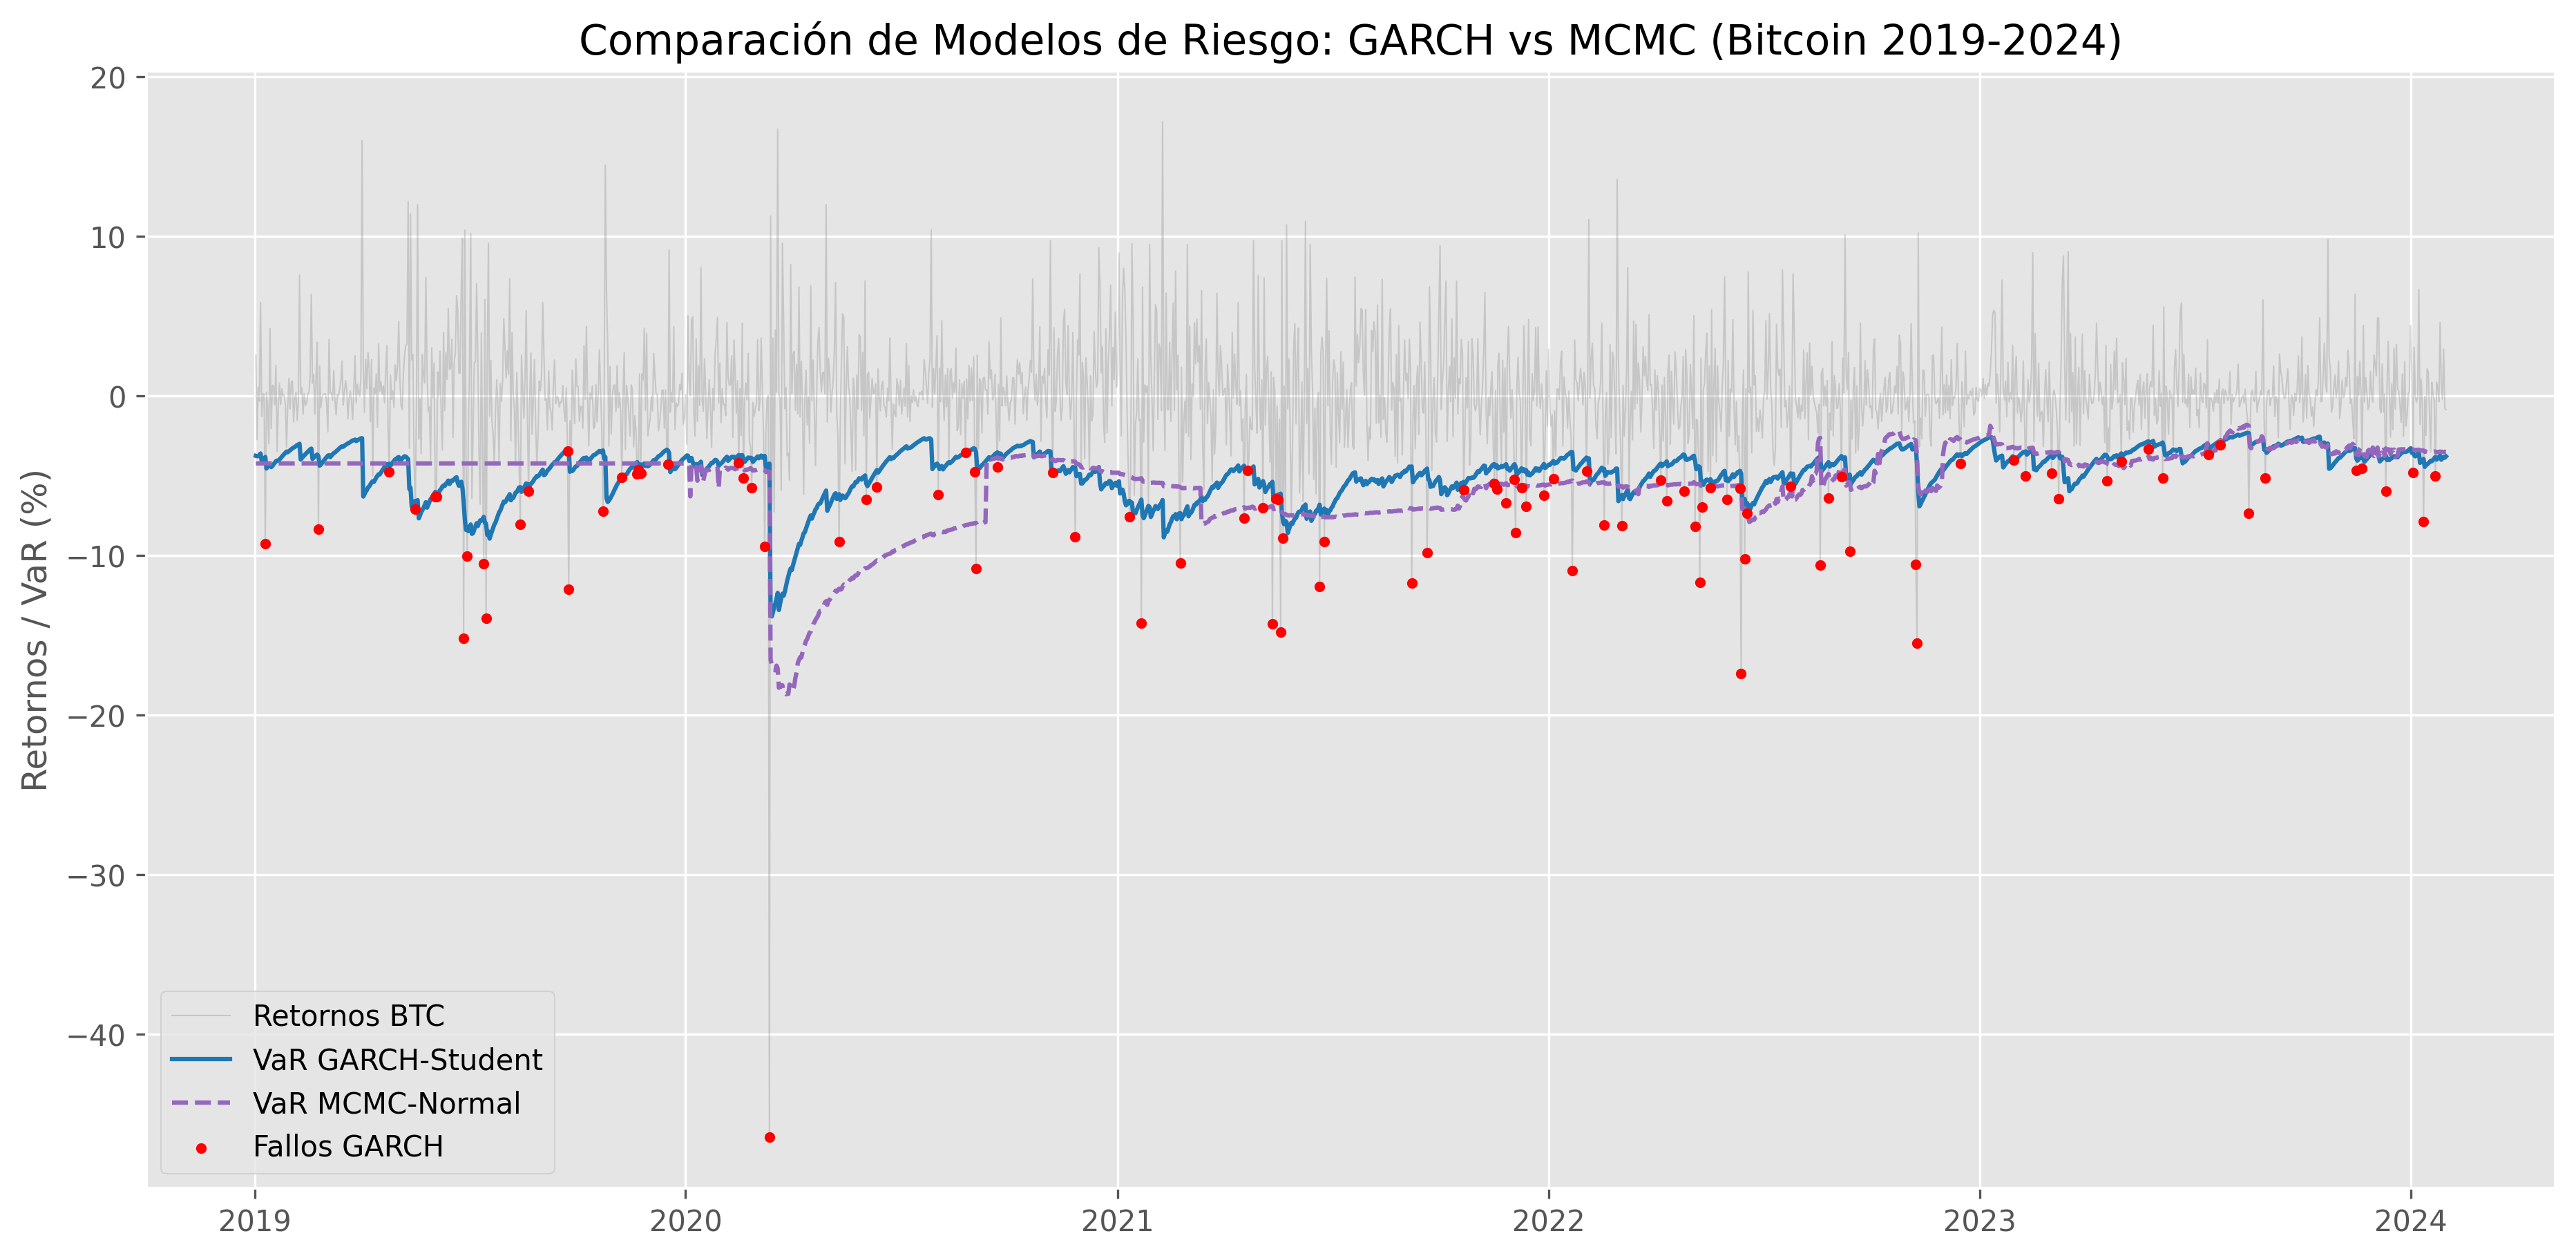
\includegraphics[width=\linewidth]{../results/figures/model_comparison.png}
  \caption{Comparación de VaR estimado por GARCH vs MCMC y retornos de Bitcoin. Se observan los ``clusters'' de volatilidad y cómo el GARCH (azul) se adapta rápidamente, mientras que el MCMC (morado) mantiene niveles más constantes por tramos.}
  \label{fig:comparison}
\end{figure}

\section{Conclusiones}

Este estudio contrastó un enfoque econométrico clásico (GJR-GARCH) frente a uno bayesiano computacionalmente intensivo (MCMC) para la gestión de riesgo en Bitcoin. Los resultados demuestran que:
\begin{enumerate}
    \item \textbf{Superioridad del GARCH:} Para la estimación diaria del VaR, el modelo GJR-GARCH con errores t-Student es superior, logrando una calibración precisa del riesgo de cola y adaptándose rápidamente a los shocks de volatilidad.
    \item \textbf{Limitaciones del Punto de Cambio Simple:} El modelo bayesiano de un solo punto de cambio resultó ser excesivamente conservador. La dinámica del Bitcoin es demasiado compleja para ser capturada por una varianza constante por tramos; requiere modelos de volatilidad estocástica (SV) o múltiples puntos de cambio.
    \item \textbf{Eficiencia de Numba:} La implementación con JIT demostró ser altamente efectiva, permitiendo inferencia bayesiana en tiempos competitivos con librerías optimizadas en C.
\end{enumerate}

Como trabajo futuro, se propone extender el modelo bayesiano a uno de Volatilidad Estocástica completa, aprovechando la infraestructura de cómputo acelerado desarrollada, para combinar la flexibilidad bayesiana con la precisión predictiva de los modelos de volatilidad variable.


\bibliography{refs.bib}

%%
%% If your work has an appendix, this is the place to put it.
% \appendix
% \section{Título del Apéndice A}
% ...

\end{document}
%%
%% End of file
